% beamer 16:9
\documentclass[aspectratio=169, 9pt, xcolor=dvipsnames]{beamer}
\usecolortheme[named=NavyBlue]{structure}
\beamertemplatenavigationsymbolsempty
\setbeamertemplate{footline}[frame number]
\usefonttheme{serif}
\setbeamertemplate{caption}[numbered]
\setbeamerfont*{itemize/enumerate subbody}{parent=itemize/enumerate body}
% math package
\usepackage{amsmath, amsthm, amssymb, booktabs, multirow, hyperref, pgffor, tabularx}
\usepackage{kotex}
\usepackage[backend=biber,style=authoryear]{biblatex}

\title{Prediction of age-structured model for SARS-CoV-2 in Seoul and Gyeonggi}
\author{Yunjeong Lee \inst{1} \and Jeongjoo Seok \inst{2}}
\institute{\inst{1} School of Mathematics and Computing (Computational Science and Engineering) \and \inst{2} School of Mathematics and Computing (Mathematics)}
\date{\today}

\addbibresource{210909_ref.bib}

\begin{document}
	
	\begin{frame}\frametitle{}
	    \maketitle
	\end{frame}

	\begin{frame}\frametitle{Data}
	    \begin{enumerate}
	    	\item Daily confirmed cases in Seoul and Gyeonggi
	    	\item Vaccine
	    	\begin{itemize}
	    		\item Daily number of vaccination for 1st dose (by age)
	    		\item Daily number of vaccination for 2nd dose (by age)
	    		\item Vaccine efficacy
	    	\end{itemize}
	    	\item Proportion of $\delta$ variant
	   	\end{enumerate}
	\end{frame}

	\begin{frame}\frametitle{Data processing}
	    \textbf{1. Daily number of vaccination for 1st dose (all ages)}
	    \begin{figure}
	    	\centering
	    	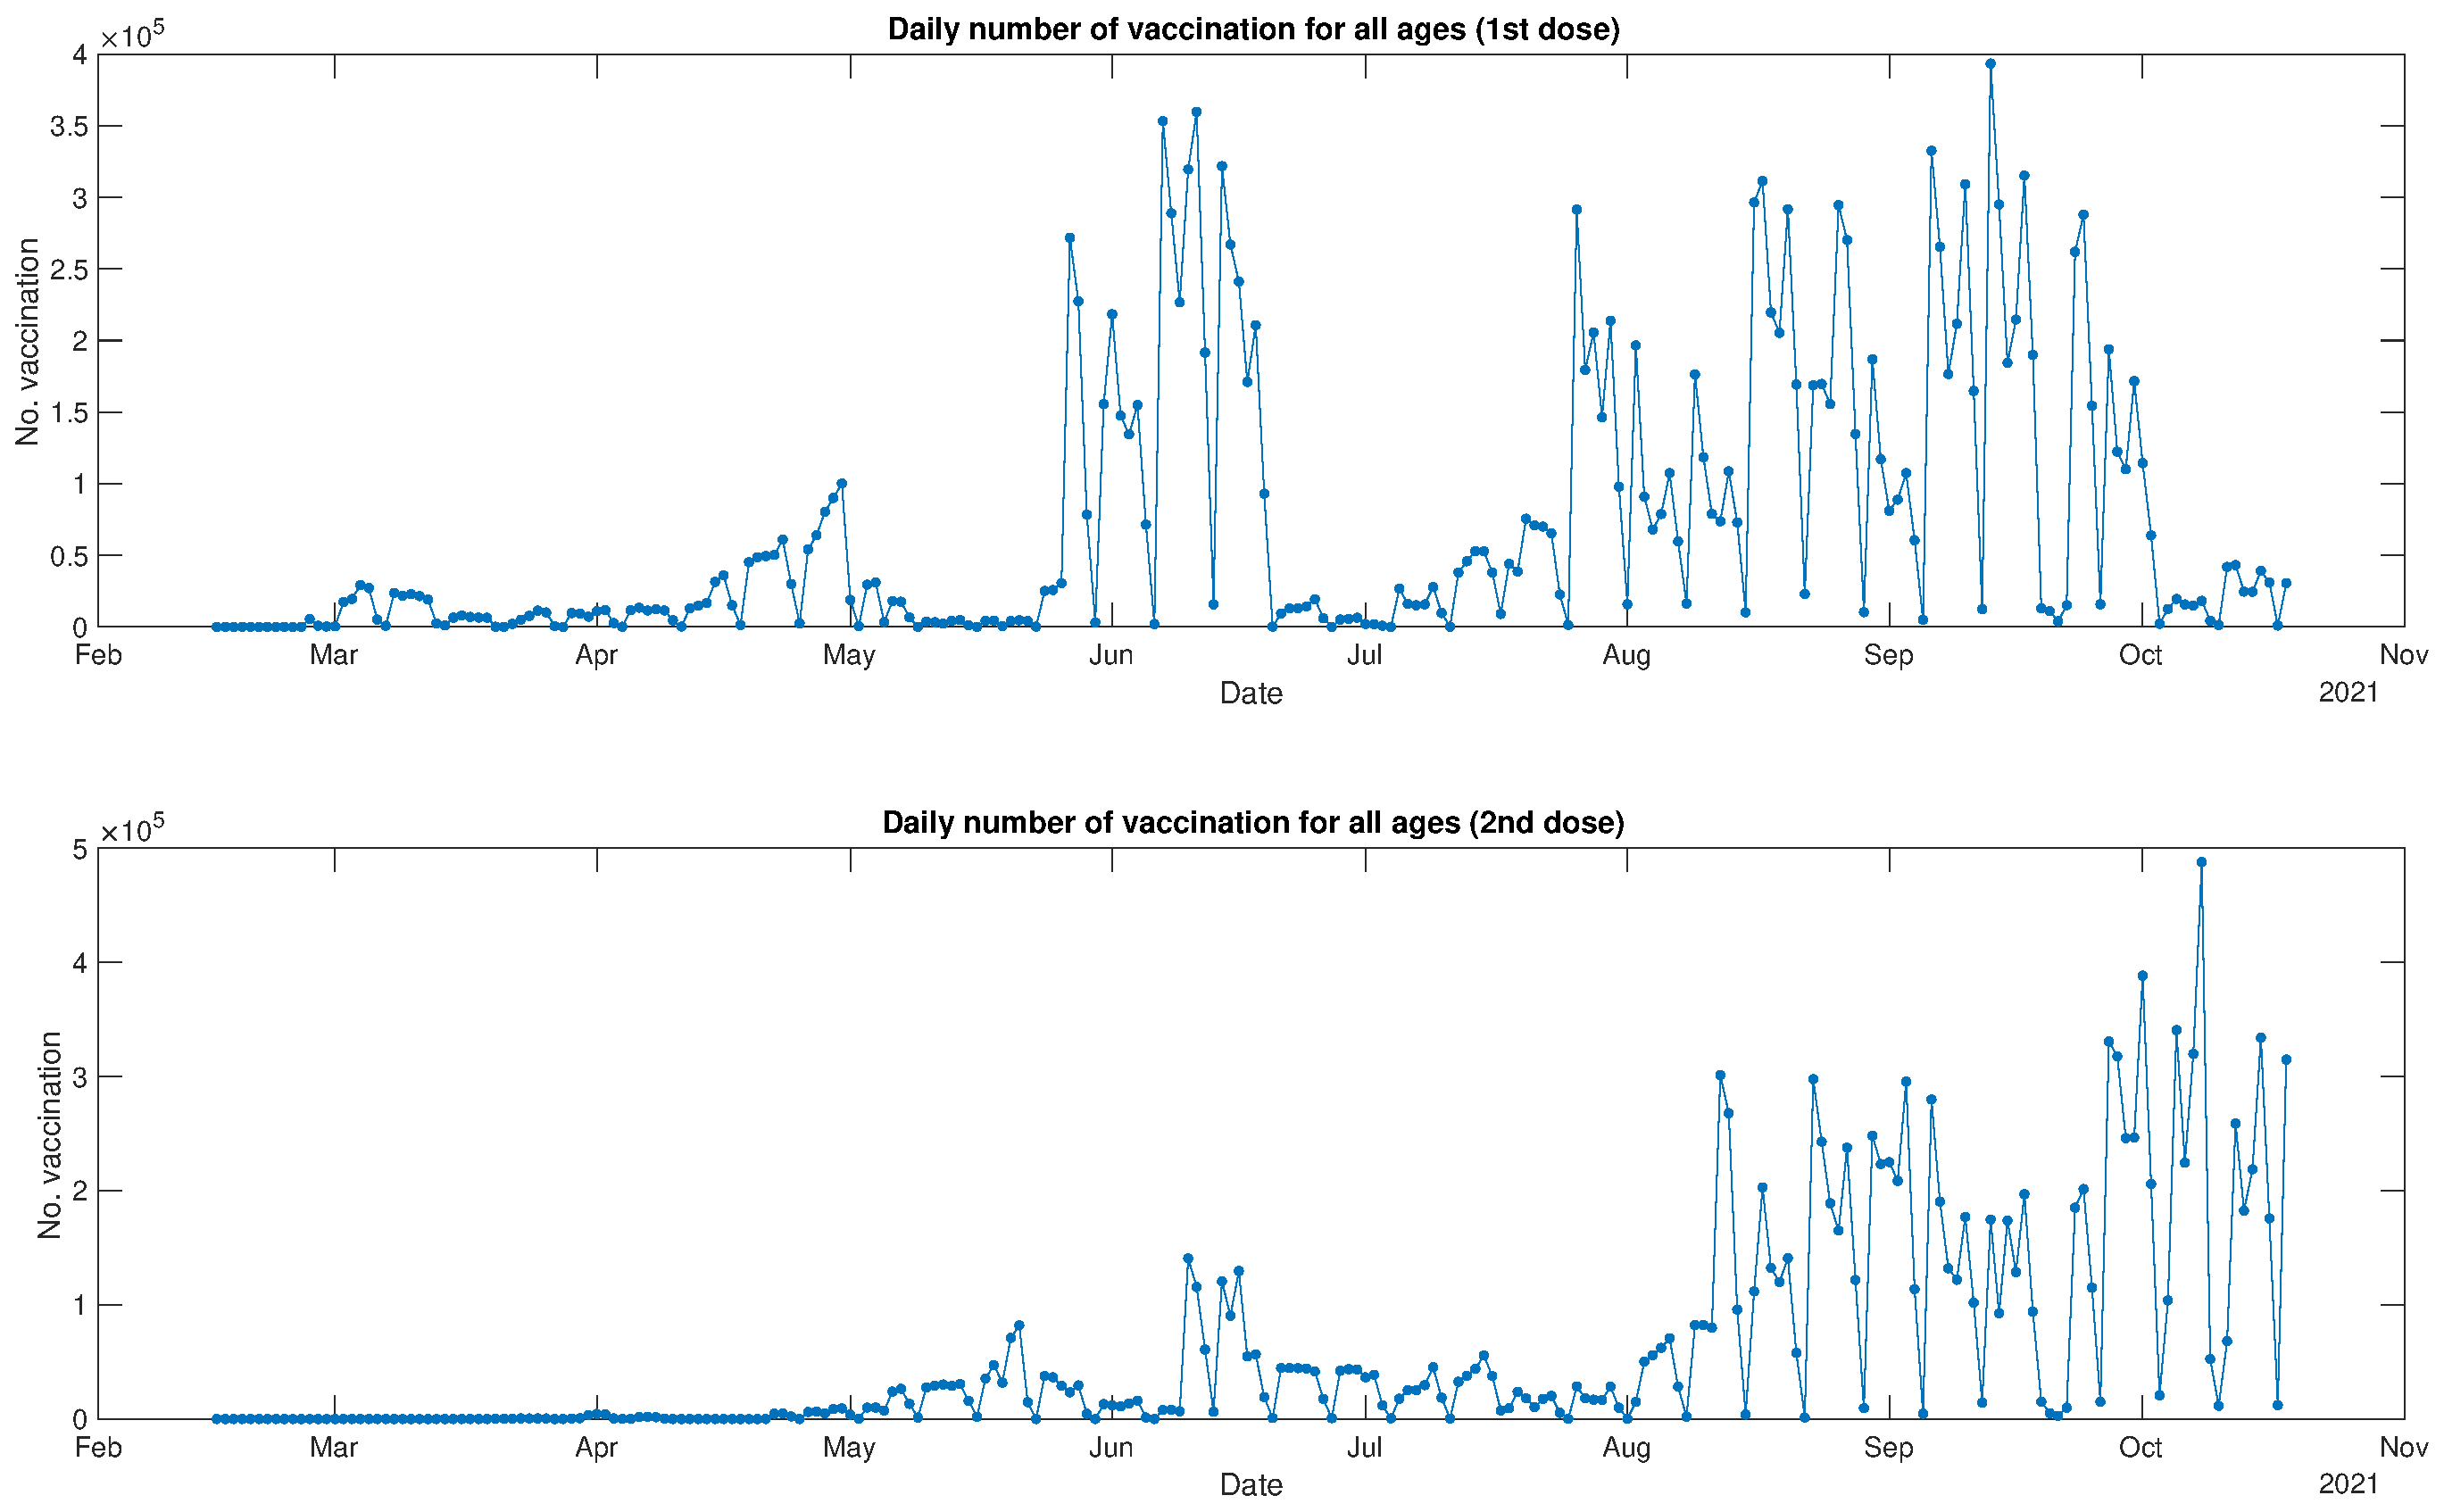
\includegraphics[width=10cm]{../results/data/vaccine_number.eps}
	    	\caption{The daily number vaccination for 1st dose and 2nd dose from 2021/02/15 to 2021/09/01}
	    \end{figure}
	\end{frame}

	\begin{frame}\frametitle{Data processing}
	    \textbf{1. Daily number of vaccination for 1st dose (by age)}
	    \begin{itemize}
	    	\item The daily number of vaccination by age is generated by the ratio between ages of vaccinated people.
	    	\item The ratio is based on KDCA reports.
	    \end{itemize}
	    \begin{figure}
	    	\centering
	    	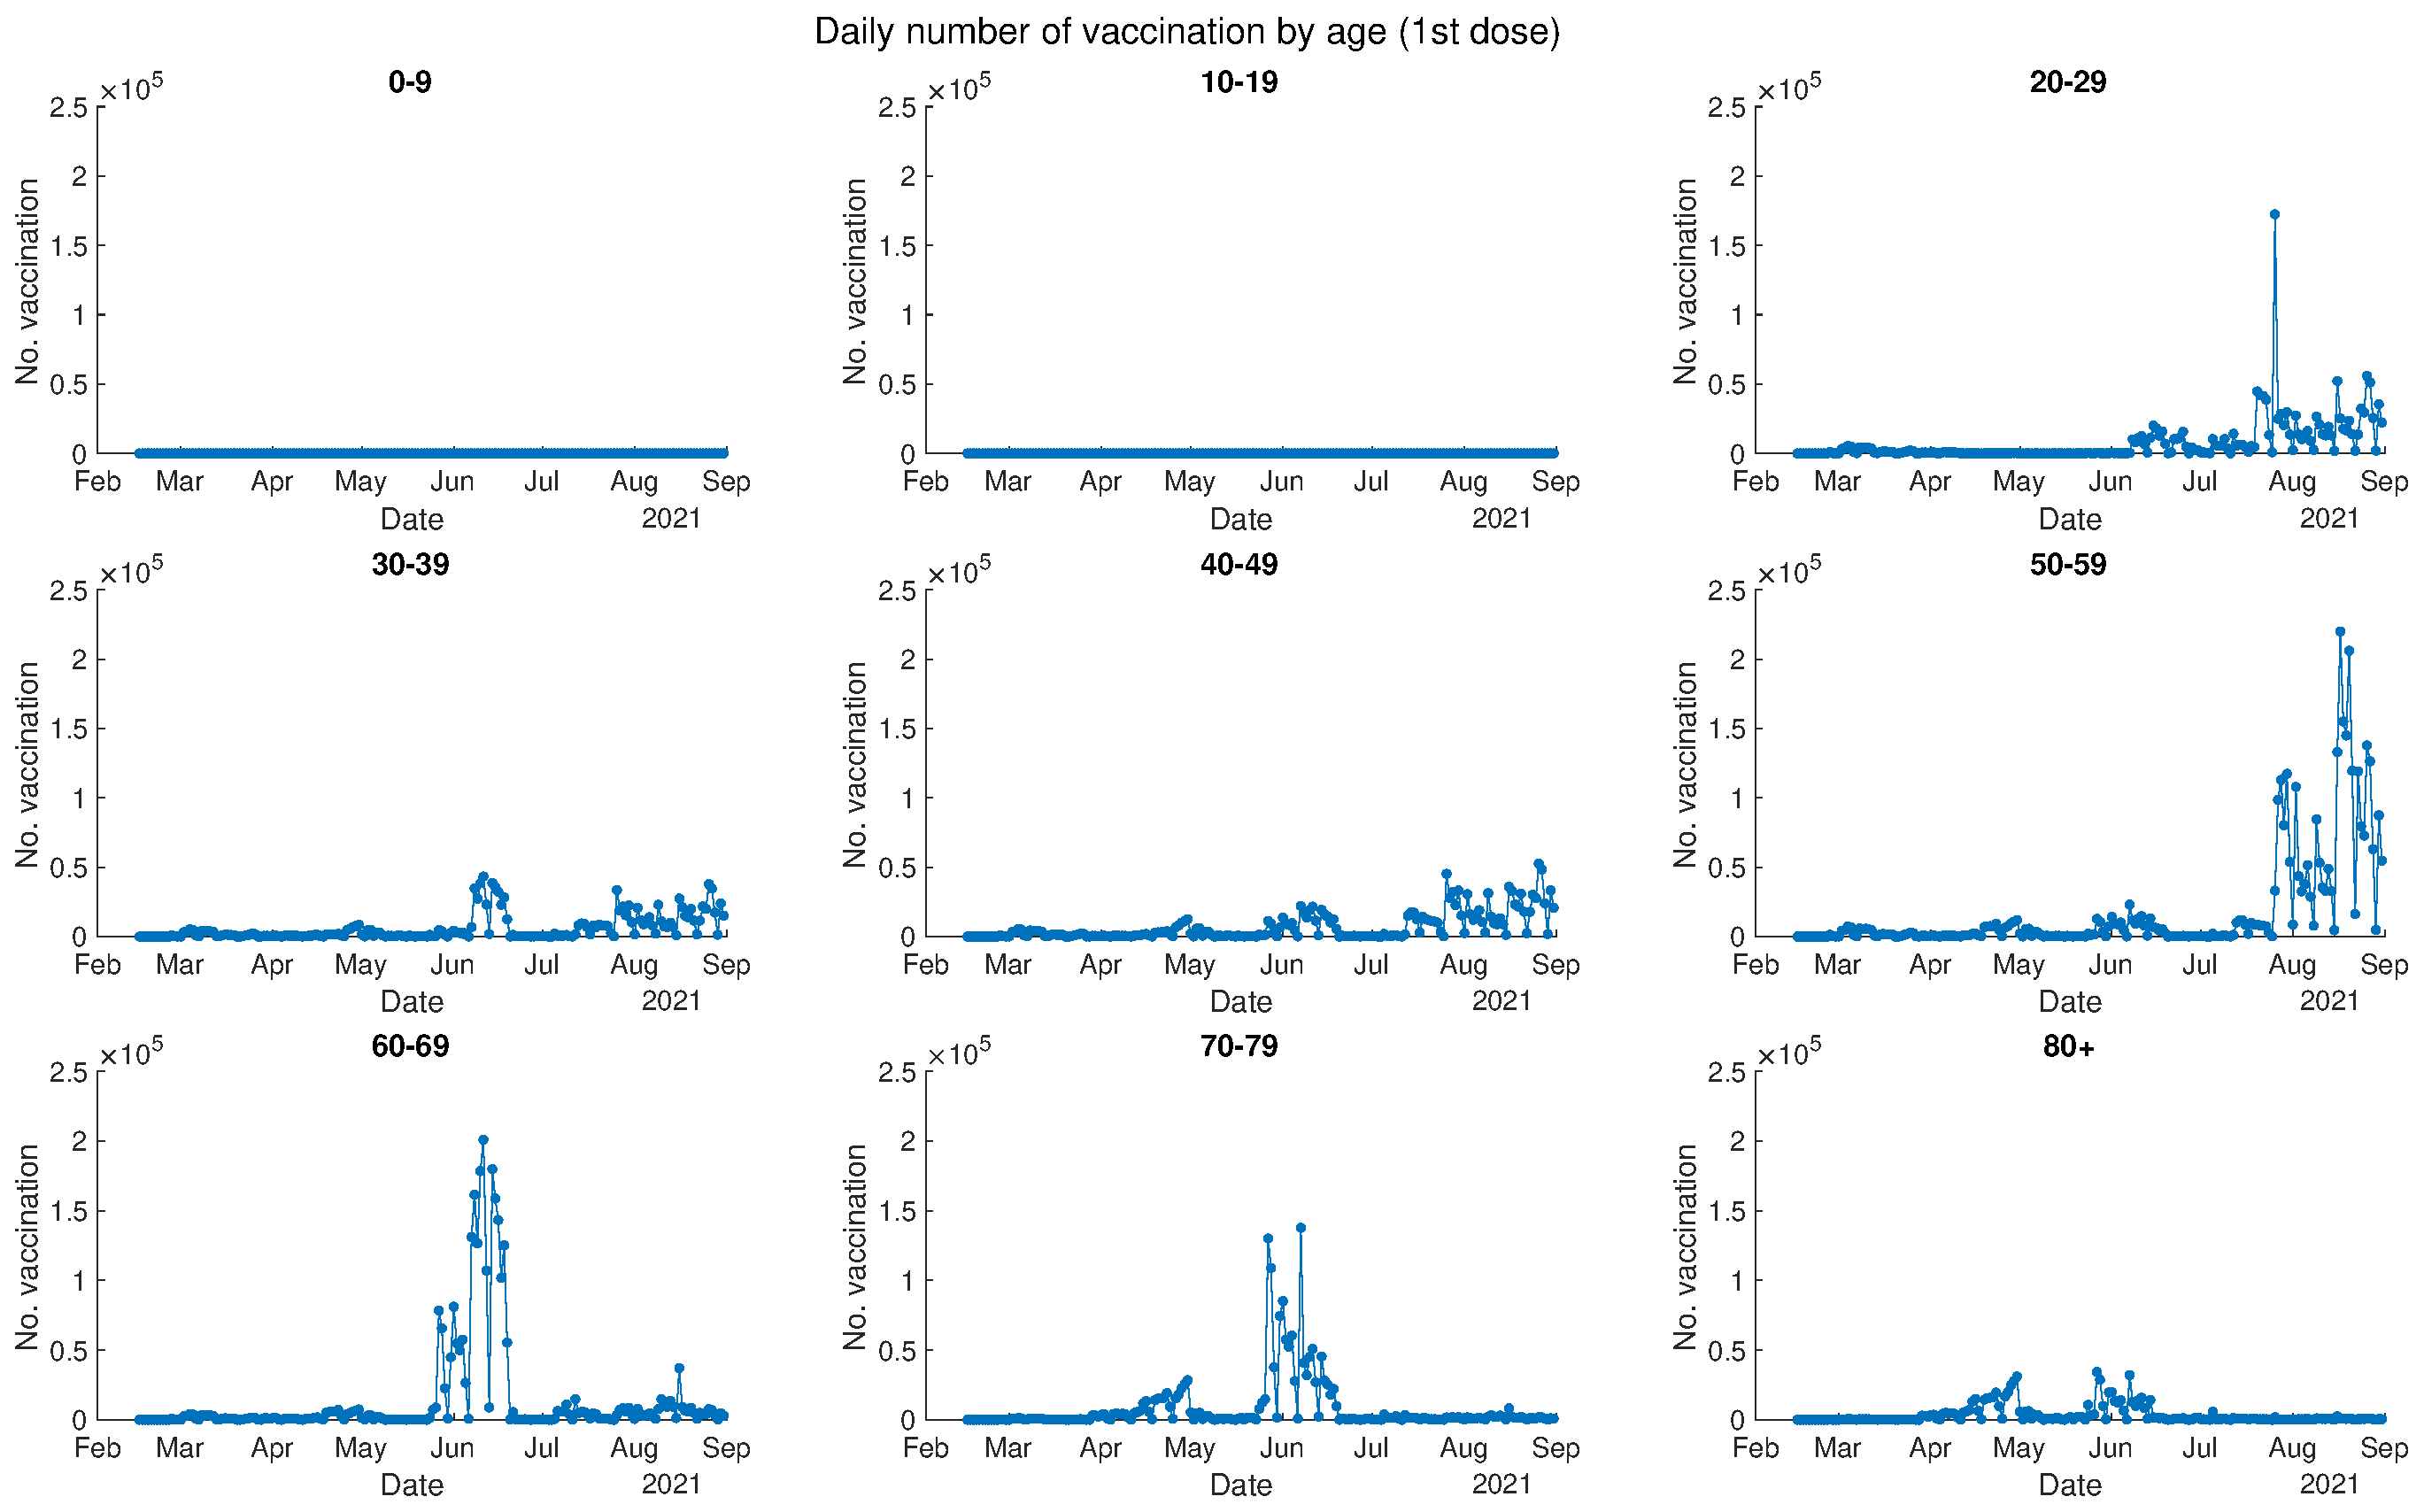
\includegraphics[width=8cm]{../results/data/vaccine_number_by_age_1st.eps}
	    	\caption{The daily number vaccination for 1st dose by age from 2021/02/15 to 2021/09/01}
	    \end{figure}
	\end{frame}

	\begin{frame}\frametitle{Data processing}
	    \textbf{2. Daily number of vaccination for 2nd dose (by age)}
	    \begin{itemize}
	    	\item The daily number of vaccination by age is generated by the ratio between ages of vaccinated people.
	    	\item The ratio is based on KDCA reports.
	    \end{itemize}
	    \begin{figure}
	    	\centering
	    	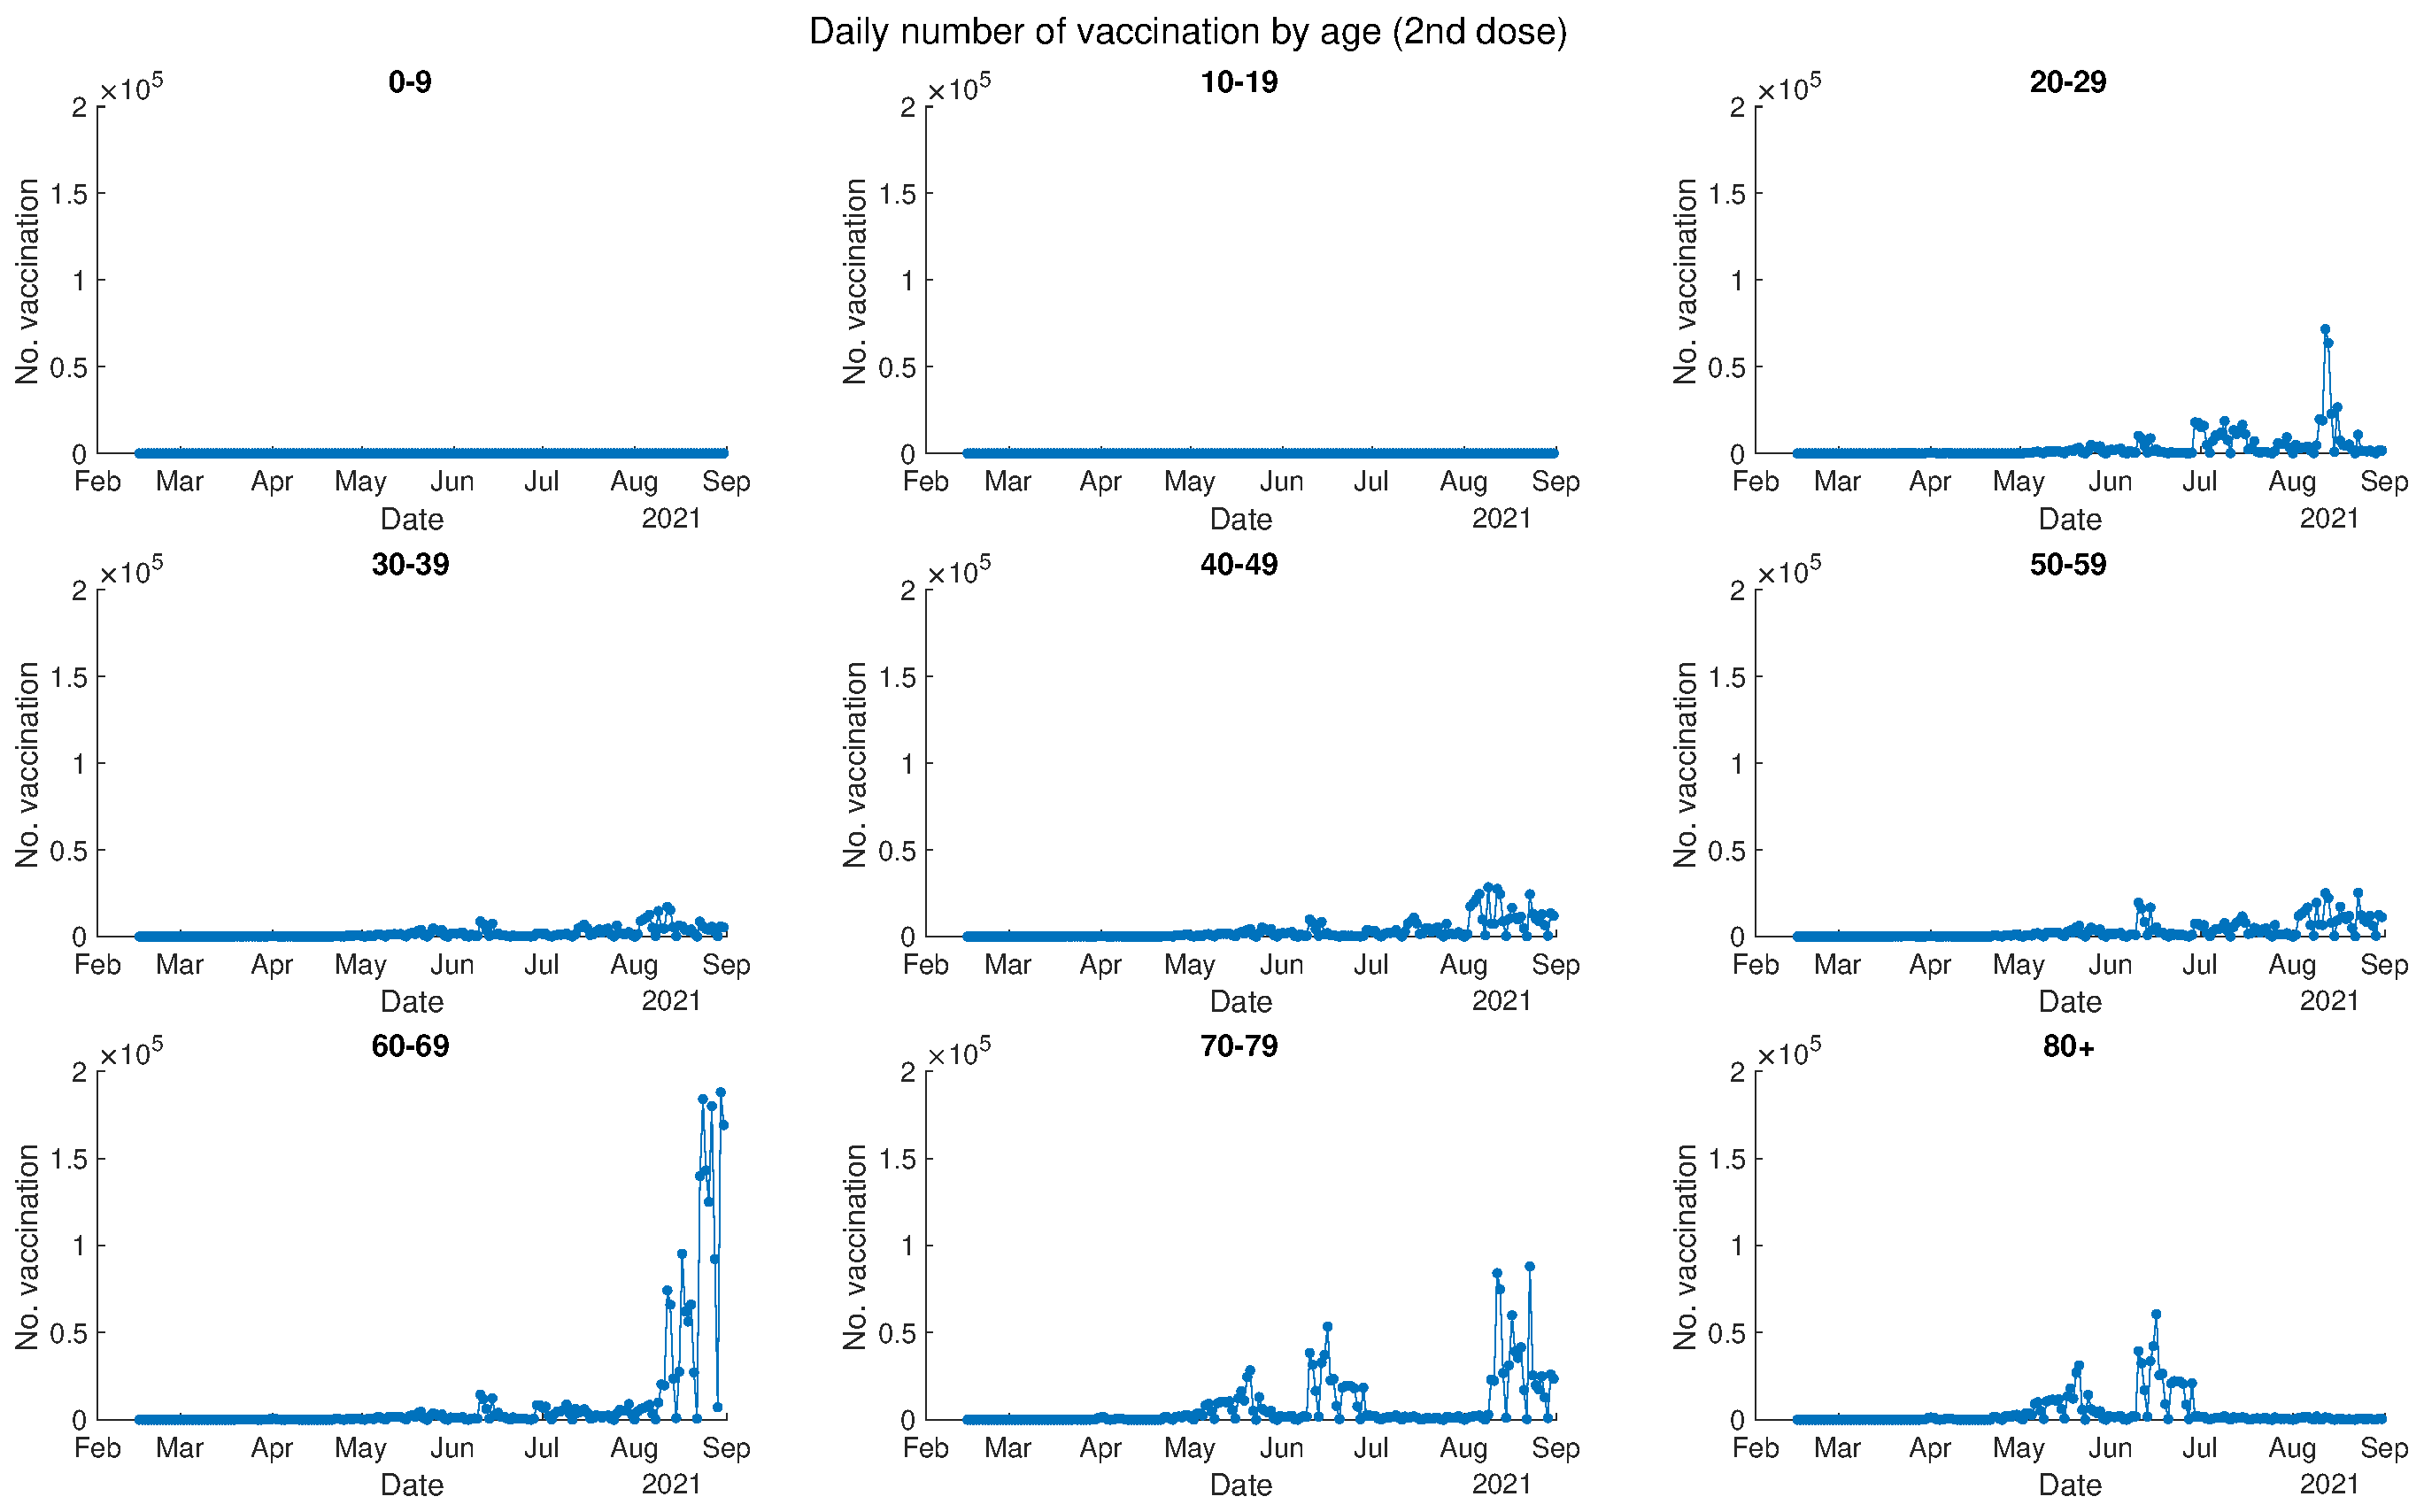
\includegraphics[width=8cm]{../results/data/vaccine_number_by_age_2nd.eps}
	    	\caption{The daily number vaccination for 2nd dose by age from 2021/02/15 to 2021/09/01}
	    \end{figure}
	\end{frame}

	\begin{frame}\frametitle{Data processing}
	    \textbf{3. Vaccine efficacy}
		\begin{itemize}
			\item The vaccine efficacies for $\alpha$ variant and $\delta$ variant are different.\footnotemark[1]
			\item We use weighted sum of vaccine efficacies where weights are based on proportion of $\delta$ variant
		\end{itemize}
		\begin{table}
			\begin{tabular}{c|crr}
				\toprule
				& \textbf{Dose} & \textbf{Astrazeneca} & \textbf{Pfizer} \\
				\midrule
				\multirow{2}{*}{$\mathbf{\alpha}$ variant} & \textbf{1st dose} & 48.7\% & 47.5\% \\
				& \textbf{2nd dose} & 74.5\% & 93.7\% \\
				\midrule
				\multirow{2}{*}{$\mathbf{\delta}$ variant} & \textbf{1st dose} & 30.0\% & 35.6\% \\
				& \textbf{2nd dose} & 67\% & 88\% \\
				\bottomrule
			\end{tabular}
			\caption{The vaccine efficacies according to the vaccine type, variant and dose.}
		\end{table}
		\footnotetext[1]{\fullcite{bernal2021effectiveness}}
	\end{frame}

	\begin{frame}\frametitle{Data processing}
	    \textbf{3. Vaccine efficacy}
		\begin{figure}
			\centering
			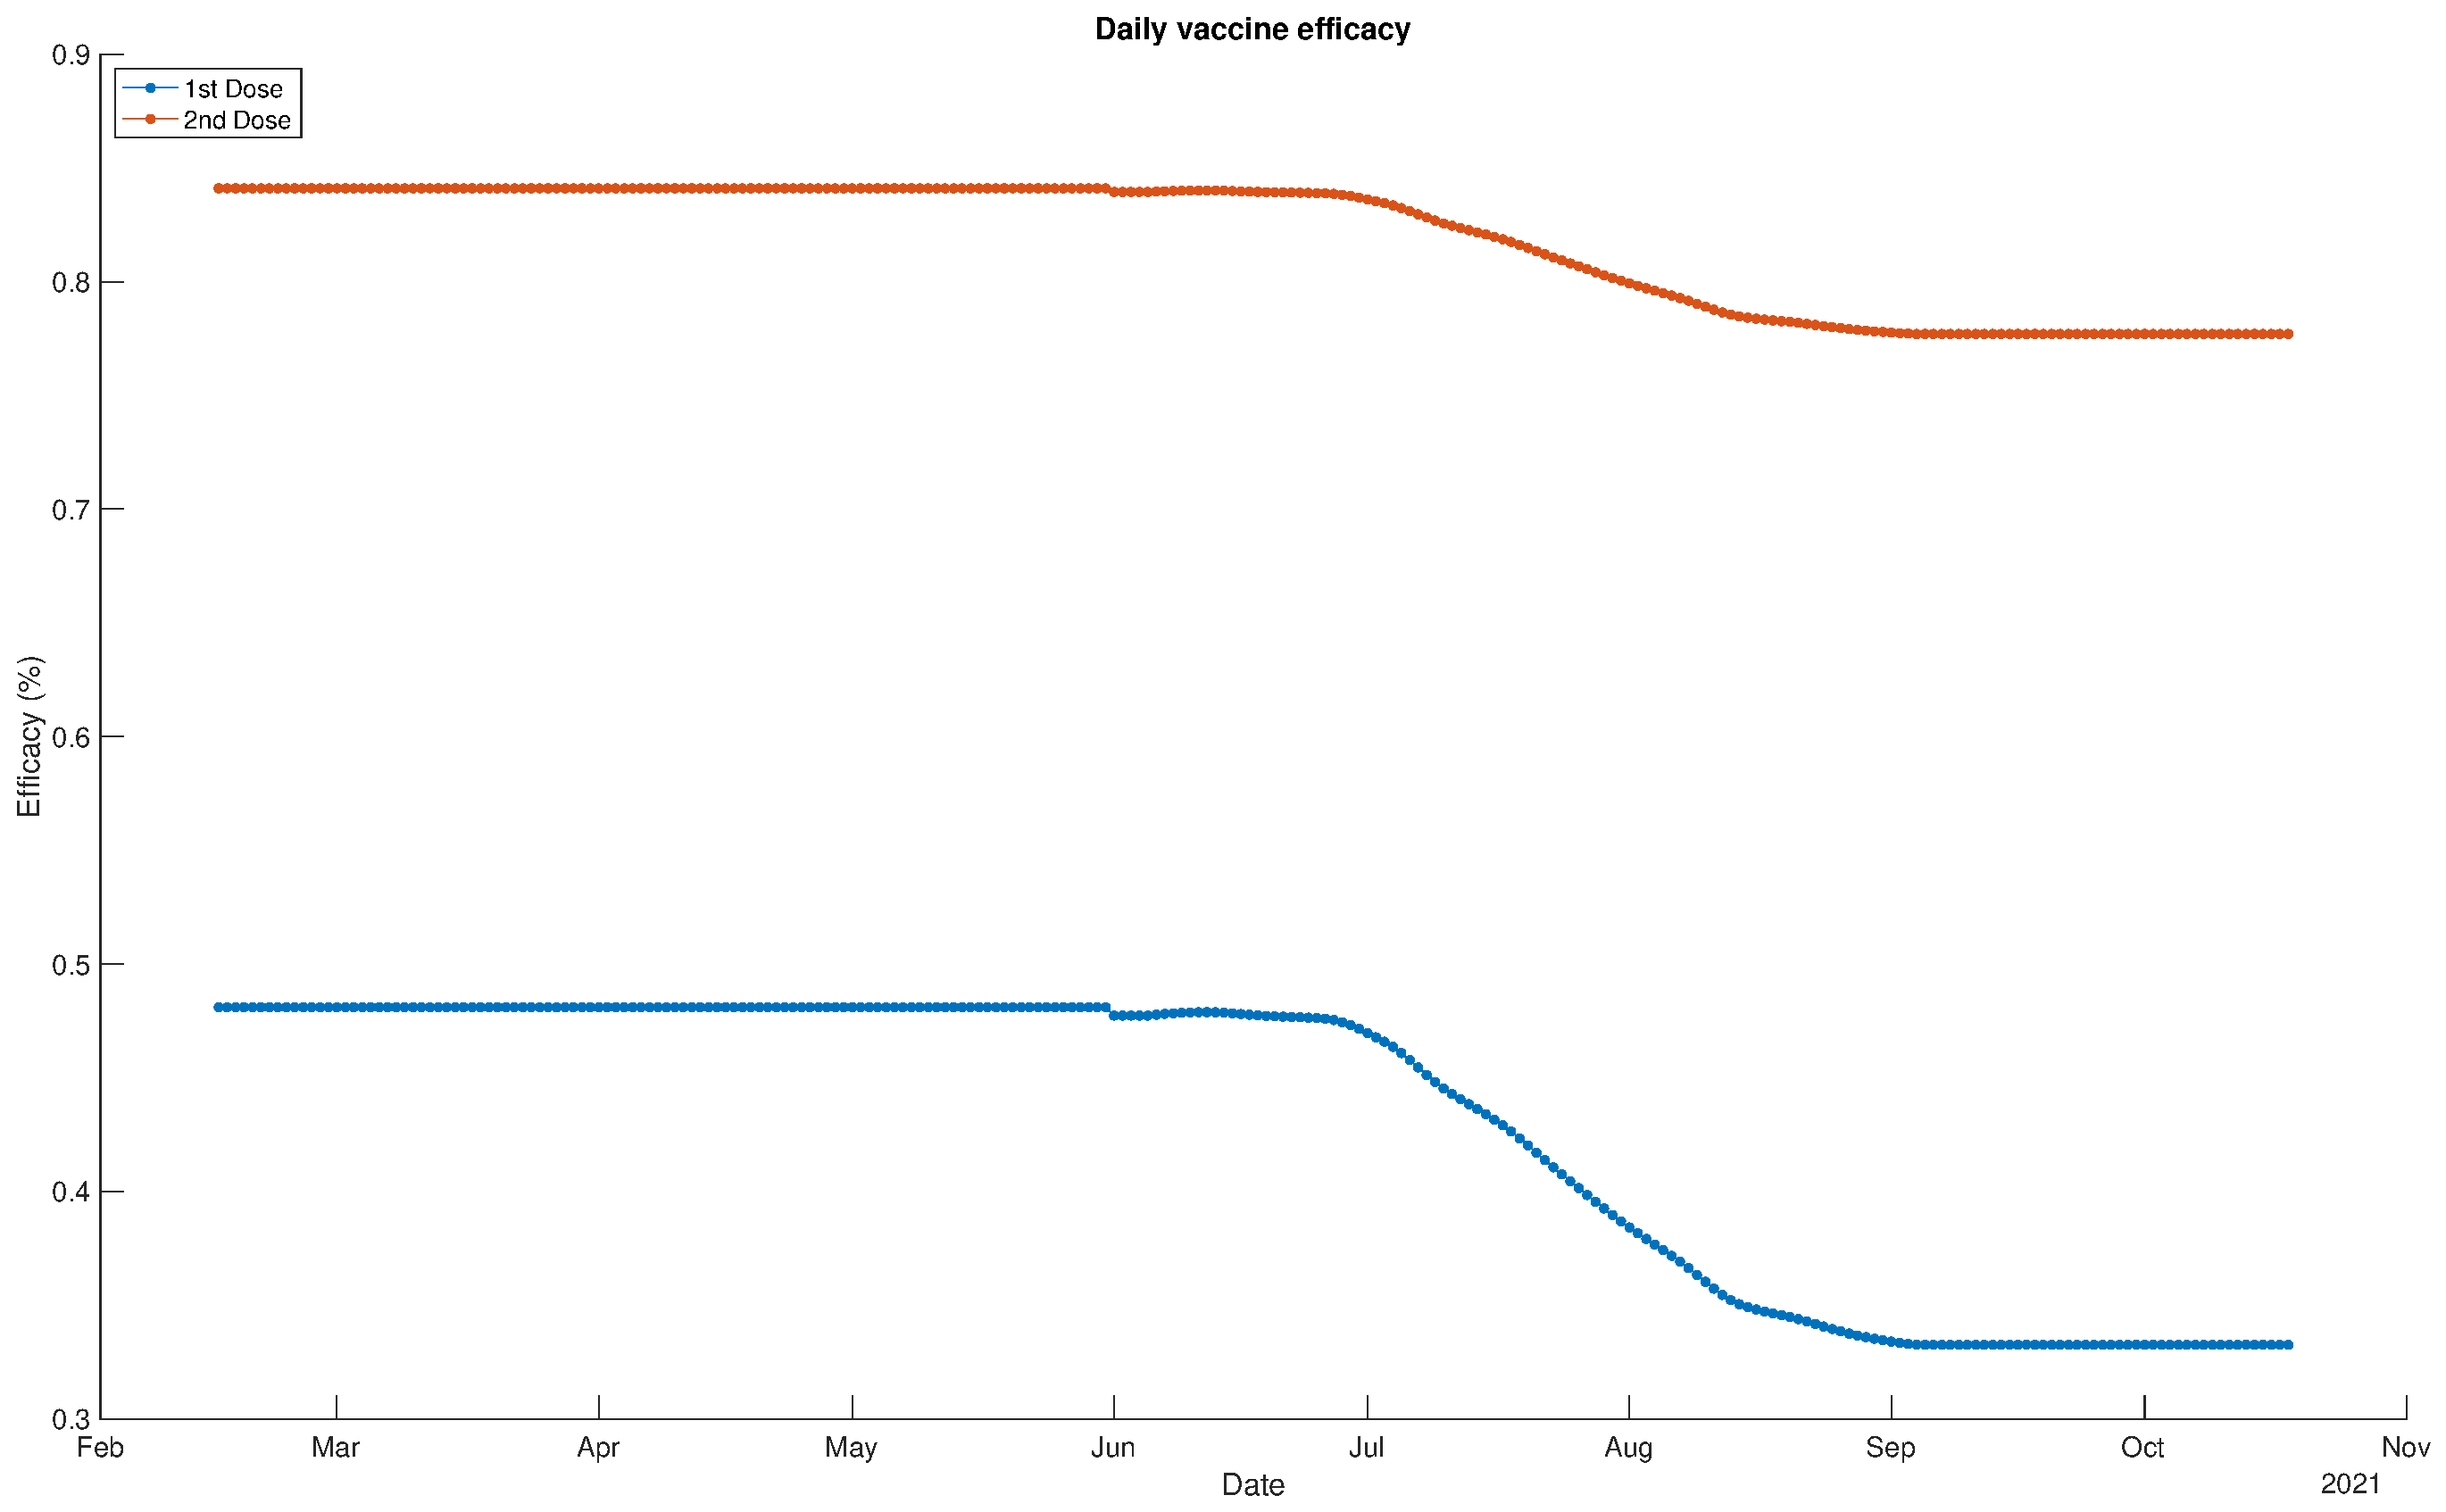
\includegraphics[width=10cm]{../results/data/vaccine_efficacy.eps}
			\caption{The estimated daily vaccine efficacy for 1st dose and 2nd dose.}
		\end{figure}
	\end{frame}

	\begin{frame}\frametitle{Data processing}
	    \textbf{4. Proportion of $\delta$ variant} \\
	    \begin{minipage}{0.3\textwidth}
	    	\begin{figure}
		    	\centering
		    	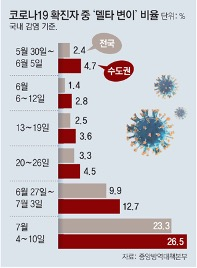
\includegraphics[width=\textwidth]{delta.jpg}
		    \end{figure}
	    \end{minipage}
	    \hfill
	    \begin{minipage}{0.6\textwidth}
	    	\begin{figure}
	    		\centering
	    		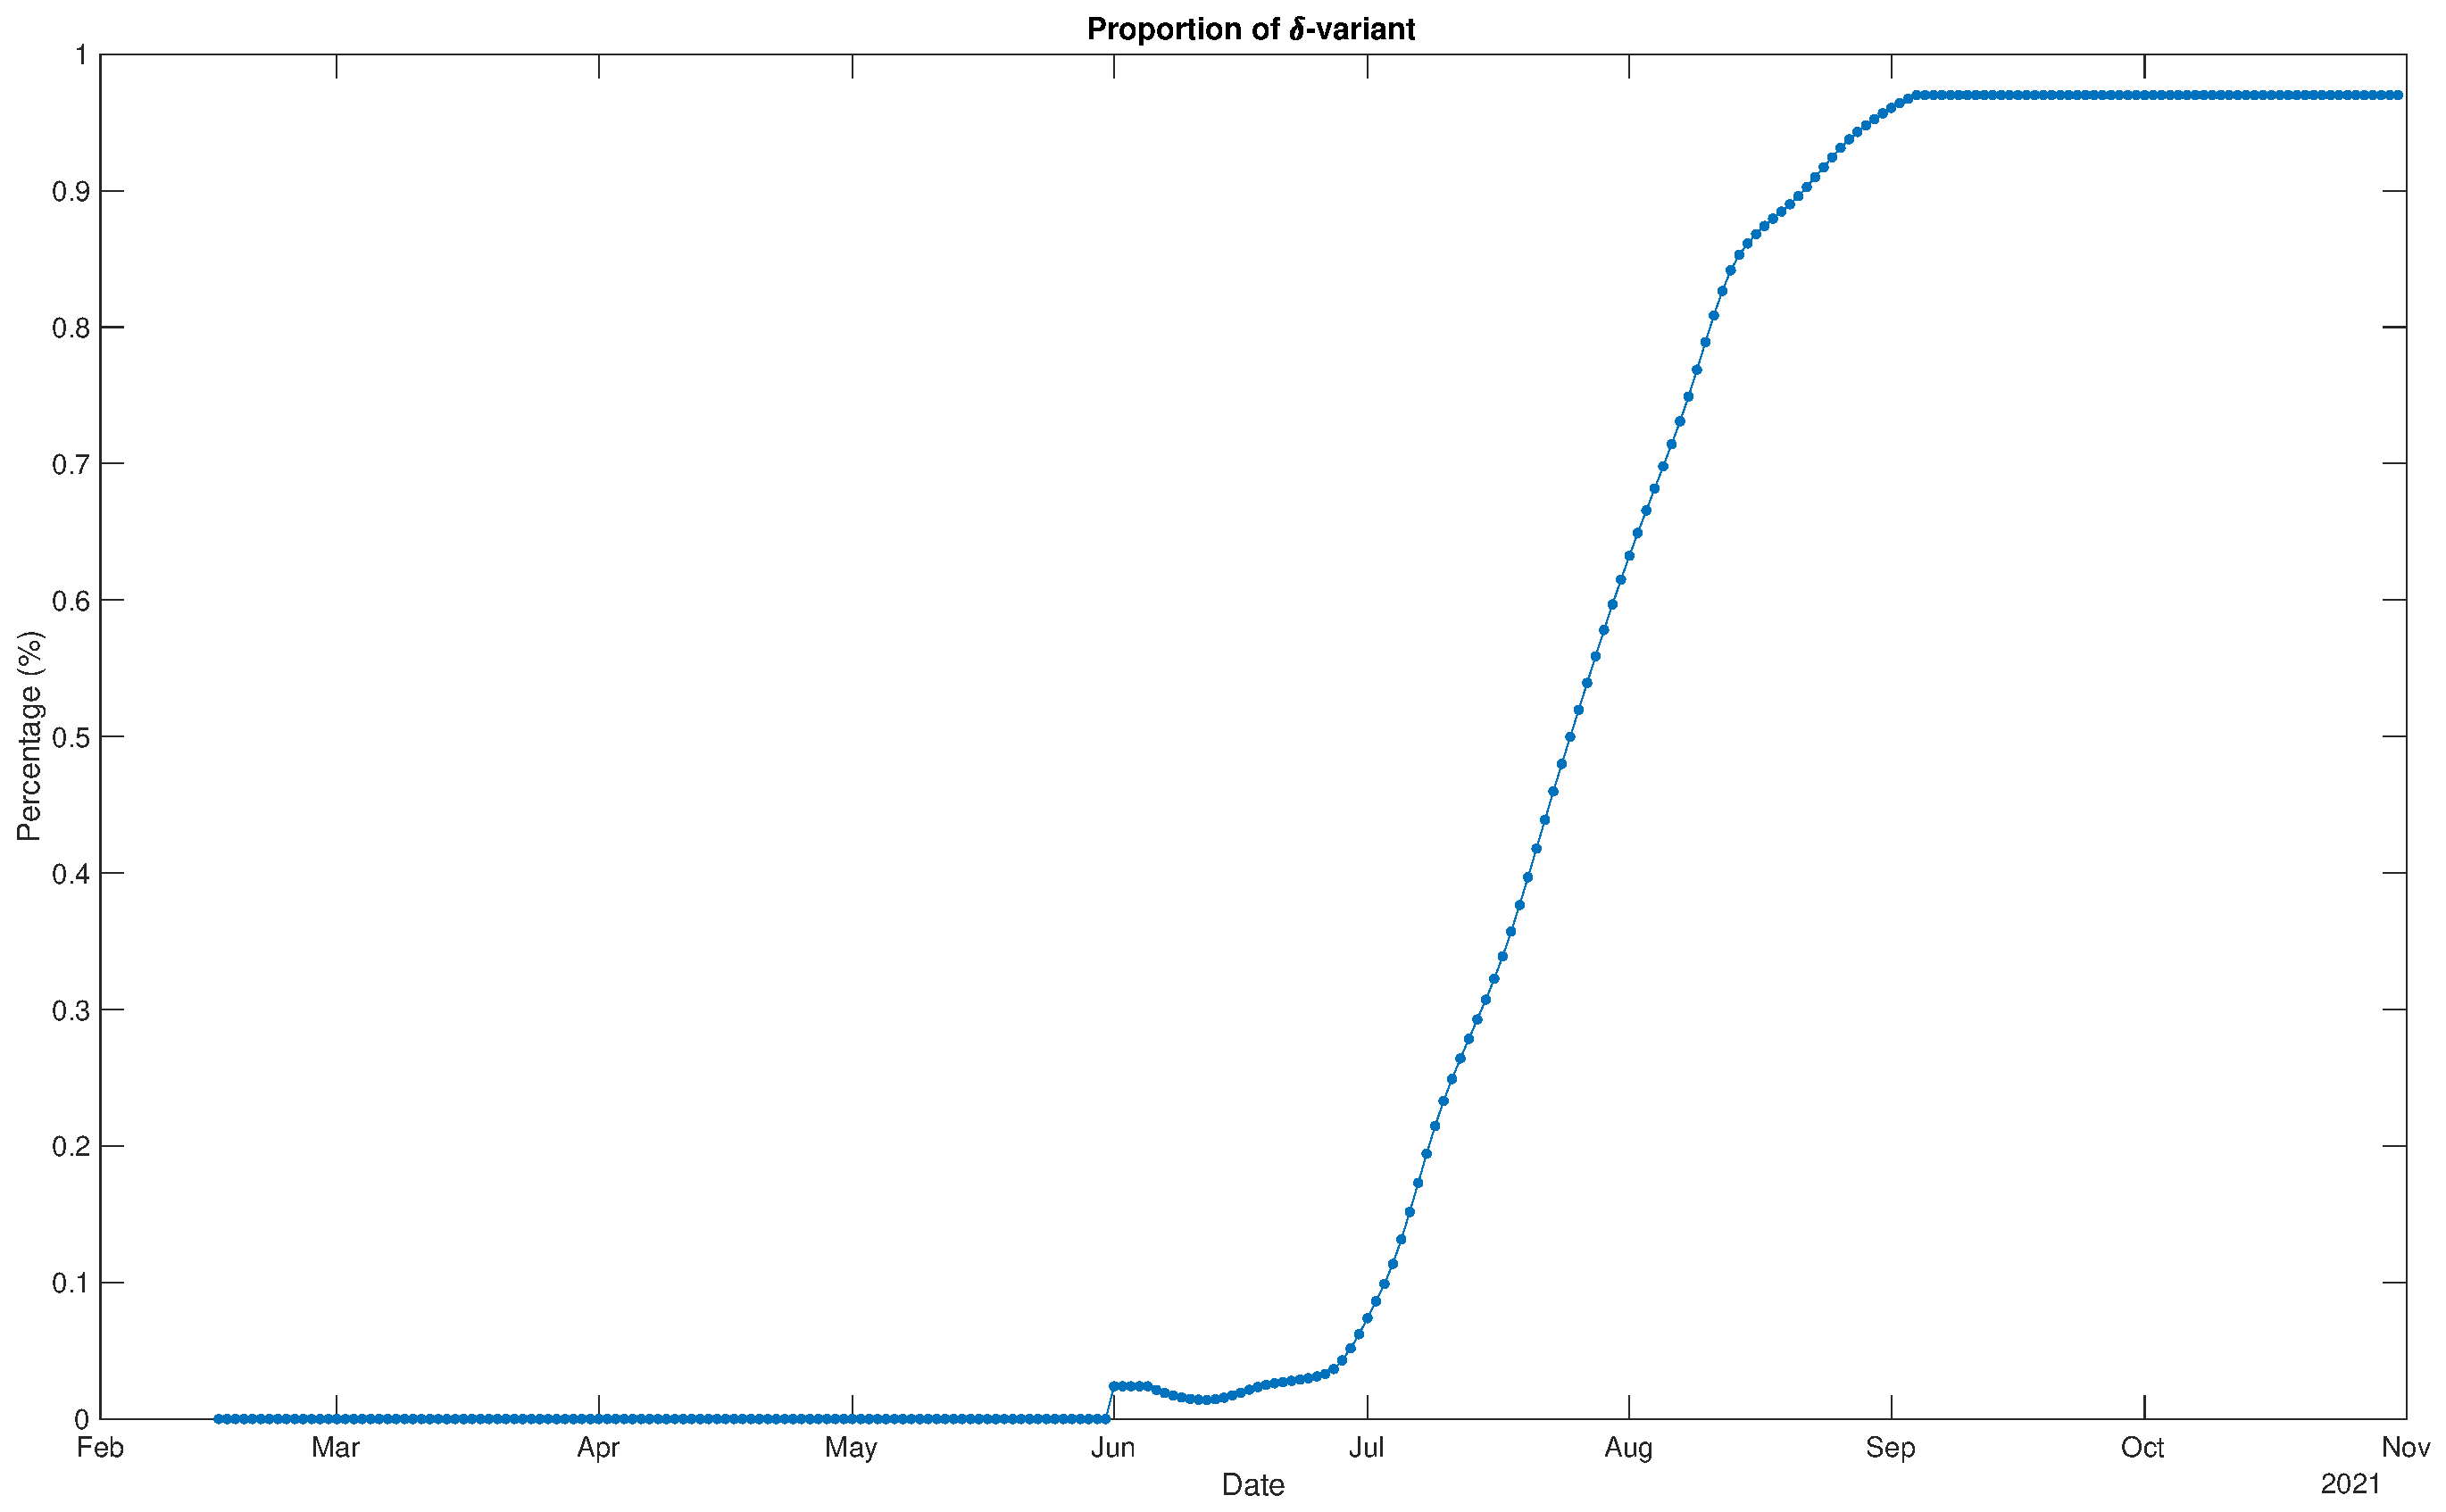
\includegraphics[width=\textwidth]{../results/data/delta_proportion.eps}
	    		\caption{Estimates of proportion of $\delta$ variant.}
	    	\end{figure}
	    \end{minipage}
	\end{frame}

	\begin{frame}\frametitle{Model}
	    \begin{figure}
	    	\centering
	    	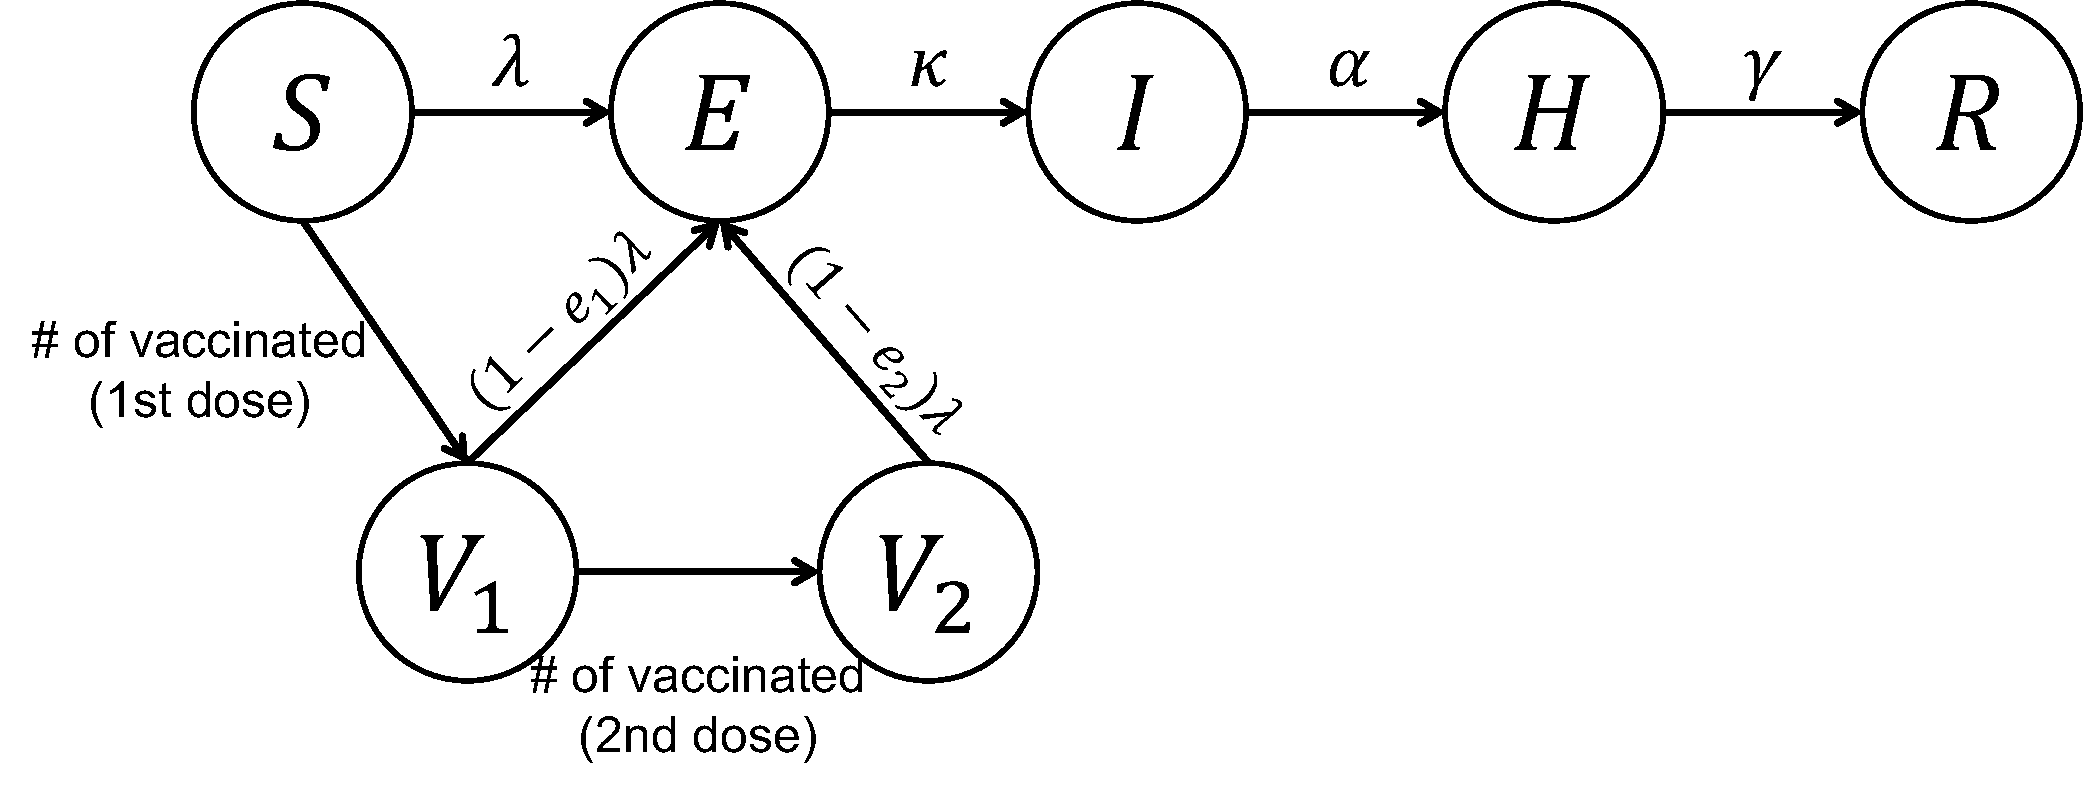
\includegraphics[width=12cm]{diagram.pdf}
	    	\caption{Diagram of age-structured model for SARS-CoV-2.}
	    \end{figure}
	\end{frame}

	\begin{frame}\frametitle{Model}
	    \begin{table}
	    	\begin{tabular}{cr}
	    		\toprule
	    		\textbf{Notation} & \textbf{Interpretation} \\
	    		\midrule
	    		$S$ & Susceptibles \\
	    		$E$ & Exposed \\
	    		$I$ & Infectious \\
	    		$H$ & Hospitalized \\
	    		$R$ & Removed (or recovered) \\
	    		$V$ & Vaccinated (between 1st dose and 2nd dose) \\
	    		$\lambda$ & Force of infection \\
	    		$\kappa$ & Latent period \\
	    		$\alpha$ & Infectious period \\
	    		$\gamma$ & Hospitalization period \\
	    		$e_1$ & Vaccine efficacy for 1st dose \\
	    		$e_2$ & Vaccine efficacy for 2nd dose \\
	    		\bottomrule
	    	\end{tabular}
	    	\caption{Definition of states and parameters.}
	    \end{table}
	\end{frame}

	\begin{frame}\frametitle{Social distancing}
		\textbf{Social distance level}
		\begin{itemize}
			\item 0.5단계 감소: transmission rate 전단계 대비 41.61\% 증가
			\item 0.5단계 증가: transmission rate 전단계 대비 30\% 감소
			\item 1단계 증가: transmission rate 전단계 대비 65\% 감소
		\end{itemize}
	    \begin{table}
	    	\begin{tabular}{lrr}
	    		\toprule
	    		\textbf{Date} & \textbf{Social distancing level} & \textbf{Change of transmission rate} \\
	    		\midrule
	    		2021/02/15-2021/06/30 & 2 &  \\
	    		2021/07/01-2021/07/11 & 1.5 & $\beta \times 1.4161$ \\
	    		2021/07/12-2021/09/01\footnotemark[2] & - & - \\
	    		\bottomrule
	    	\end{tabular}
	    	\caption{The change of transmission rate according to the social distancing level from 2021/02/15 to 2021/09/01.}
	    \end{table}
	    \footnotetext[2]{It will be changed according to the experiments.}
	\end{frame}

	\begin{frame}\frametitle{Definition of $\lambda$}
		\textbf{Motivation}
	    \begin{itemize}
	    	\item In general, $\lambda(t)$ is defined by $W \times I(t)$ where $W$ is the WAIFW matrix, and $I(t)$ is the number of infectious at time $t$.
	    	\item To reflect the non-pharmaceutical intervention, we consider time-dependent $W(t)$.
	    \end{itemize}
	    \vspace{0.5cm}
	    \textbf{Definition of WAIFW matrix} \\
	    Let $p(t)$ and $SD(t)$ be the proportion of $\delta$ variant and proportionate of the corresponding social distancing level at time $t$. Let $C(t)$ be the contact rate at time $t$.
	    \begin{itemize}
	    	\item $W(t) = \left((1 - p(t) + p(t) \delta\right) \times \beta \times SD(t) \times C(t)$
	    \end{itemize}
	\end{frame}

	\begin{frame}\frametitle{Experiments}
		\textbf{Baseline scenario}
	    \begin{table}
	    	\begin{tabular}{crrr}
	    		\toprule
	    		 & \textbf{2/15-6/30} & \textbf{7/1-7/11} & \textbf{7/12-9/26} \\
	    		\midrule
	    		\textbf{사회적 거리두기} & 2단계 & 1.5단계 & 2.5단계 \\
	    		\bottomrule
	    	\end{tabular}
	    	\caption{The social distancing level of baseline scenario}
	    \end{table}
	    \textbf{Experiments} \\
	    Combination of following settings
	    \begin{itemize}
	    	\item 사회적 거리두기 (2021/09/27-2021/12/31)
	    	\begin{itemize}
	    		\item 현행 유지
	    		\item 0.5단계 완화: $1.4306(=1/0.699)$배
	    		\item 1단계 완화: $2.8571(=1/0.35)$배
	    	\end{itemize}
	    	\item 등교 관련
	    	\begin{itemize}
	    		\item 현행 유지
	    		\item contact이 거리두기 0.5단계 완화 수준으로 증가: $1.4161$배
	    		\item contact이 거리두기 1단계 완화 수준으로 증가: $2.0053(=1.4161^2)$배
	    	\end{itemize}
	    \end{itemize}
	\end{frame}

	\foreach \sd in {same, 0.5, 1} {
		\foreach \sc in {same, 0.5, 1} {
			\begin{frame}\frametitle{사회적 거리두기 완화 수준: \sd단계\, \& 등교로 인한 contact 증가 수준: \sc}
			    \begin{figure}
			    	\centering
			    	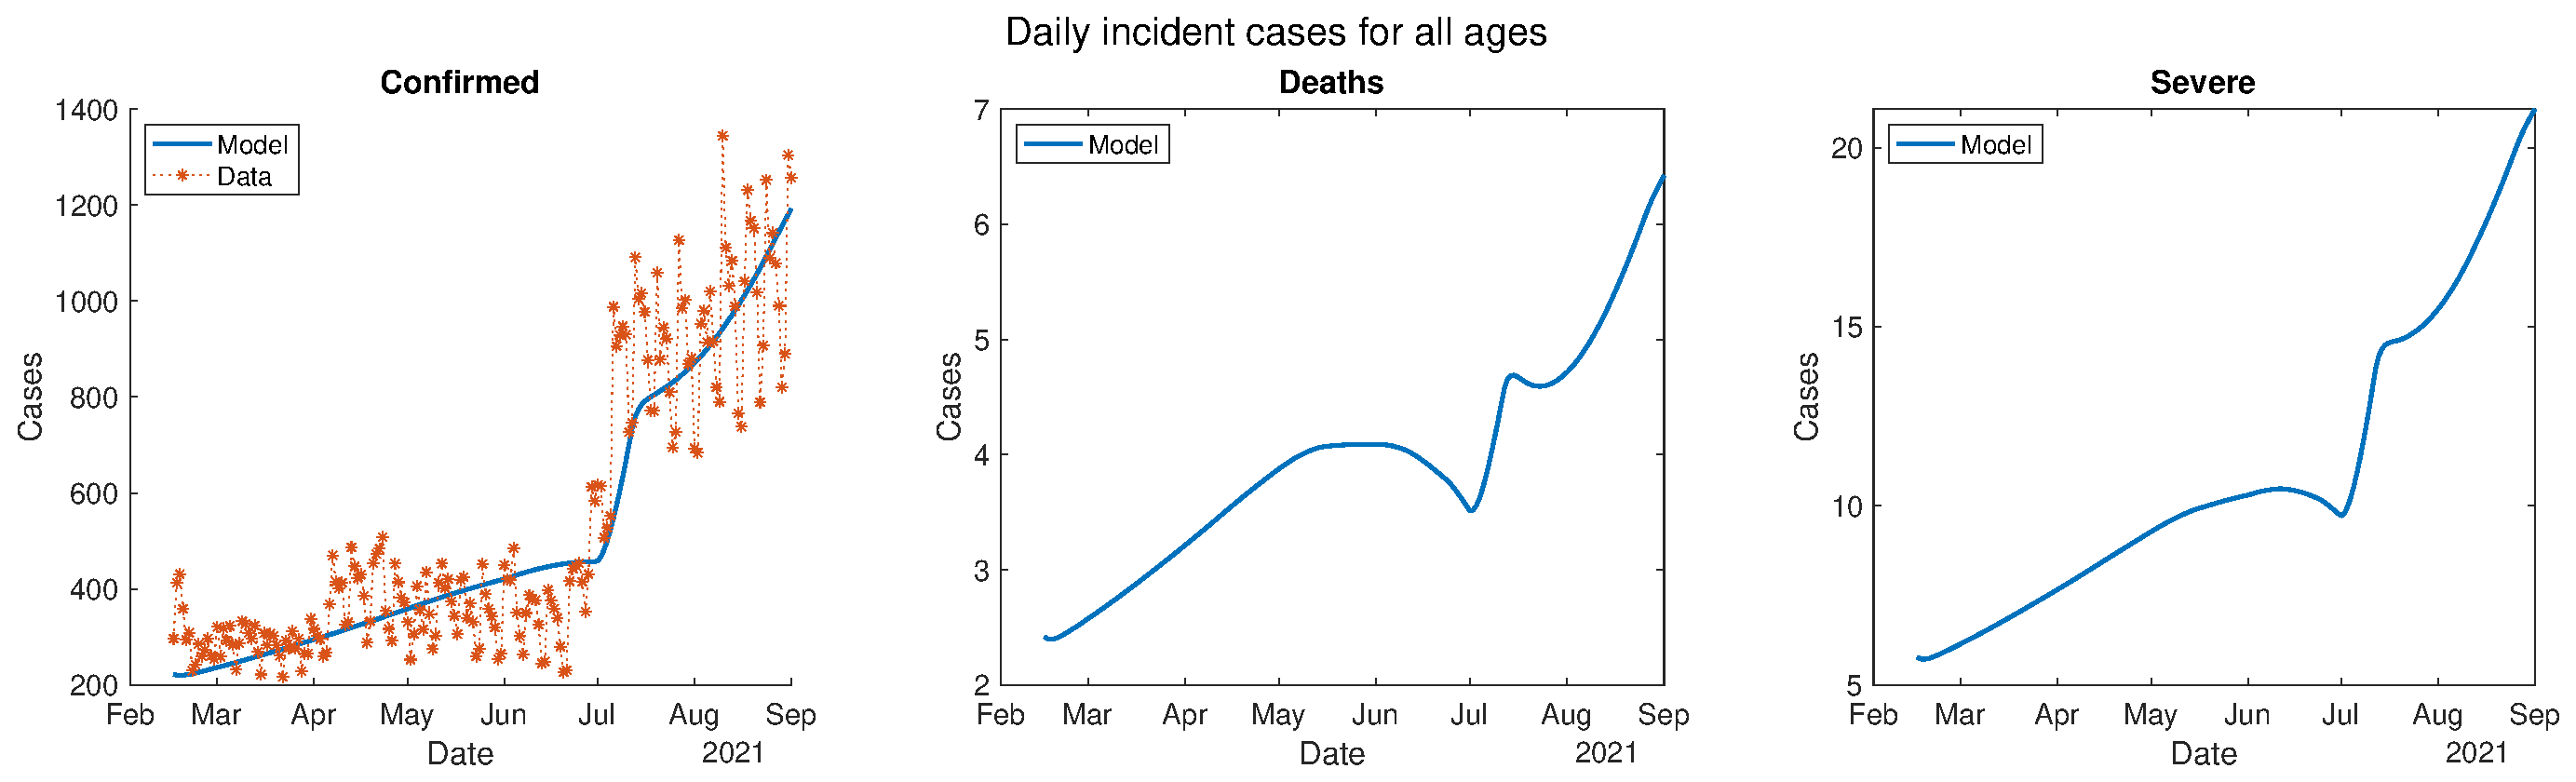
\includegraphics[width=11cm]{../results/predict_exp_3_sd3_\sd_school_\sc/daily_all_age.eps}
			    	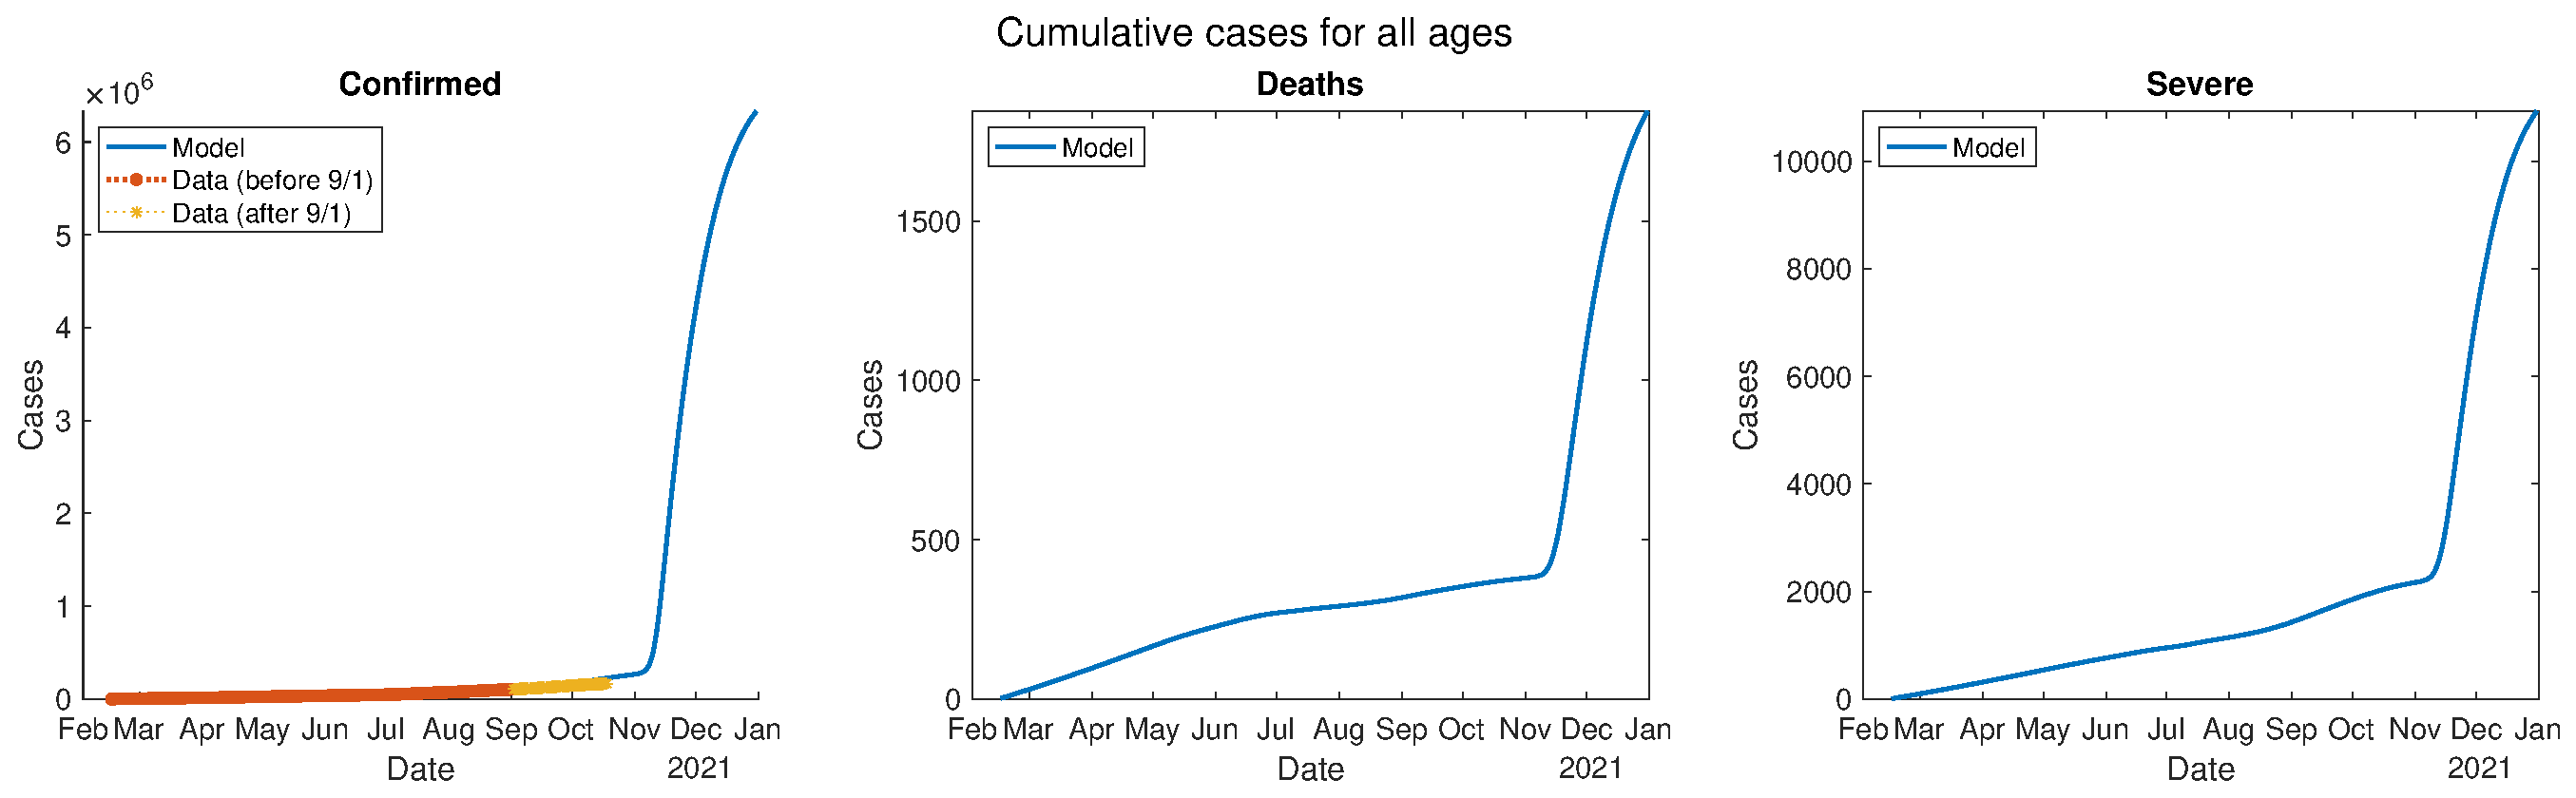
\includegraphics[width=11cm]{../results/predict_exp_3_sd3_\sd_school_\sc/cumul_all_age.eps}
			    	\caption{The model prediction and data for daily confirmed cases (top) and cumulative confirmed cases (bottom).}
			    \end{figure}
			\end{frame}

			\begin{frame}\frametitle{사회적 거리두기 완화 수준: \sd단계\, \& 등교로 인한 contact 증가 수준: \sc}
			    \begin{figure}
			    	\centering
			    	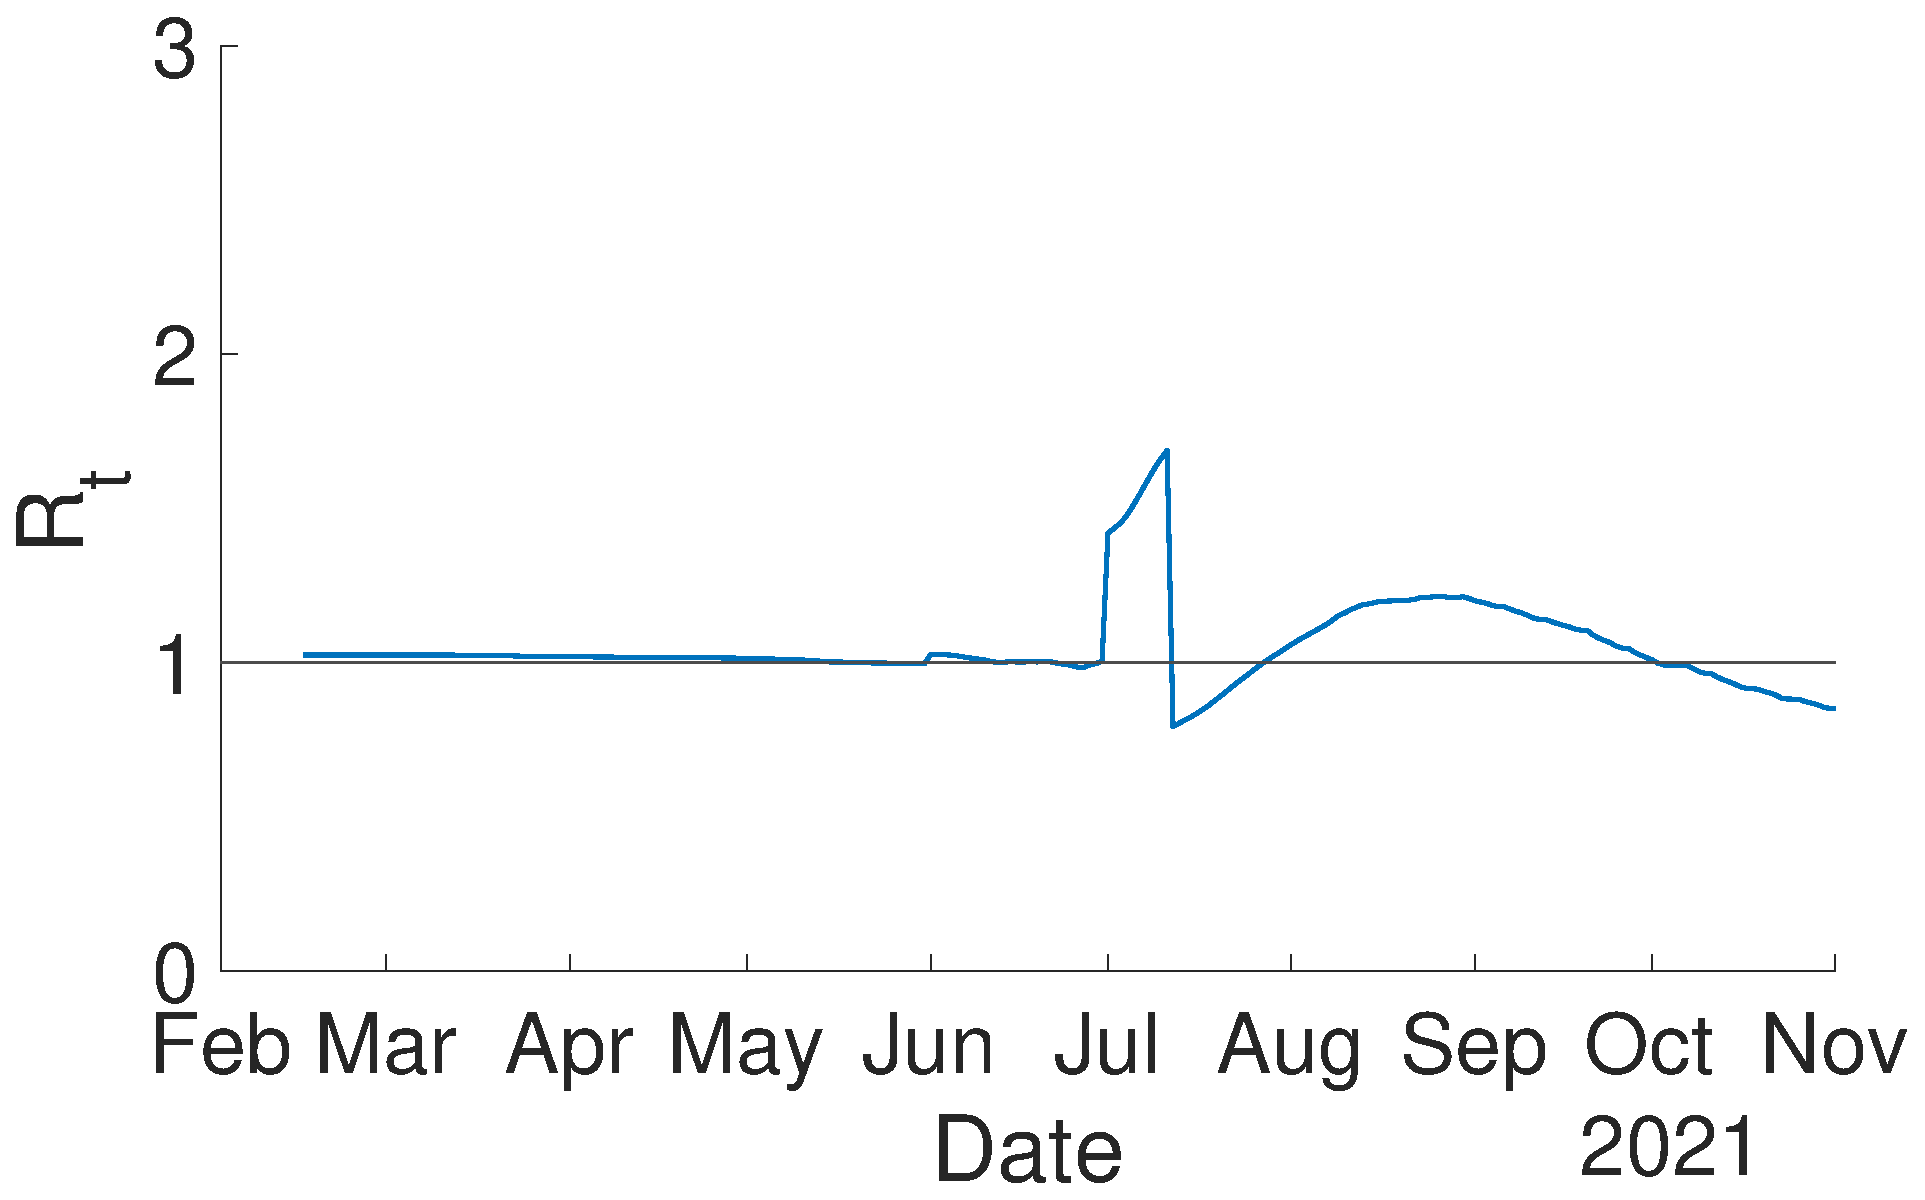
\includegraphics[width=10cm]{../results/predict_exp_3_sd3_\sd_school_\sc/rep_num.eps}
			    	\caption{The estimated reproduction number from 2021/02/15 to 2021/09/01.}
			    \end{figure}
			\end{frame}
		}
	}

\end{document}